\section{Ein Kapitel}
\label{sec:kapitel}

\subsection{Literatur zitieren}

Mit dem \texttt{\textbackslash{}cite} Befehl sieht es folgenderma"sen aus:
\cite{Lehnfeld2014} oder auch \cite{Vidal2013}.

Mit dem Befehl \texttt{\textbackslash{}citet} bzw. \texttt{\textbackslash{}textcite} stattdessen so:
\textcite{Lehnfeld2014}.

Wenn nur die Namen der Autoren benötigt werden, kann
\texttt{\textbackslash{}citeauthor} benutzt werden: \citeauthor{Lehnfeld2014}.

Und hier noch ein Buch \cite{Brucker2007} und ein Konferenzartikel 
\cite{Huang2010}.

\subsection{Gleichungen referenzieren}
\label{sec:gleichungen-referenzieren}

Die folgende Gleichung hat das Label \texttt{eq:polyederformel}.
Somit kann sie, wie alle anderen gelabelten Objekte, mit
\texttt{\textbackslash{}ref\{eq:polyederformel\}}
referenziert werden.
Mit dem Befehl \texttt{\textbackslash{}eqref} 
erh"alt man die Referenz in runden Klammern: 
Gleichung~\eqref{eq:polyederformel}.

\begin{equation}
  \label{eq:polyederformel}
  E - K + F = 2
\end{equation}

Sei $x \in \mathbb{R}$. Nun betrachte die Summe $\sum_{i=1}^n \sum_{\ell = 0}^{i} x^\ell$ ... und folgende Gleichungen
% Gleichungen mit alignment, jeweils mit und ohne Numerierung
\begin{align}
a &= b + c + d      \label{eqn:important1} \\
  &= b + c + e - f  \nonumber \\
  &= xy             \label{eqn:important2}
\end{align}

Aus Gleichungen \eqref{eqn:important1} und \eqref{eqn:important2} folgt ...

\begin{mytheorem}
	Dies ist ein Theorem.
\end{mytheorem}
\begin{proof}
	Dies ist ein Beweis.
\end{proof}

\subsection{LP-Formulierung}
\label{subsec:lp}

\begin{align}
\max 	&& \sum_{i = 1}^n c_i x_i \label{eq:zielf}\\
\text{s.t.} && \sum_{i = 1}^n w_i x_i &\leq W&& \label{eq:c1}\\
	&& x_i & \in \{0, 1\} && (i = 1, \ldots, n)
\end{align}
In der Zielfunktion \eqref{eq:zielf} wird irgend etwas mininimiert ...



\subsection{Tabellen}

\begin{table}[!htbp] \centering
\small
\begin{tabular}{|r|r||r|r|r||r|r|r||r|r|r||} \hline
& & \multicolumn{3}{c||}{$\alpha=0$} & \multicolumn{3}{c||}{$\alpha=0.5$} & \multicolumn{3}{c||}{$\alpha=0.8$}\\
$m$ & $n$ & \# ver & gap & time &  \# ver & gap & time &  \# ver & gap & time  \\  \hline
2 & 10   & 5  & 0	& 1	& 5 & 0   	& 0	& 5 &0		& 0\\
2 & 50   & 3  & 0.01	& 721	& 3 & 0.01	& 742	& 0 &0.84	& 1800\\
2 & 100  & 4  & 0.00	& 367	& 4 & 0.00	& 491	& 0 &0.35	& 1800\\
2 & 150  & 5  & 0	& 40	& 5 & 0		& 811	& 0 &0.27	& 1800\\
3 & 10   & 5  & 0	& 0	& 5 & 0		& 0	& 5 &0 		& 0\\
3 & 50   & 3  & 0.01	& 1094	& 1 & 0.03	& 1752	& 0 &2.12	& 1800\\ 
3 & 100  & 5  & 0	& 243	& 0 & 0.22	& 1800	& 0 &2.23	& 1800\\
3 & 150  & 4  & 0.00	& 894	& 0 & 0.15	& 1800	& 0 &3.18	& 1800 \\
5 & 10   & 5  & 0	& 0	& 5 & 0 	& 0	& 5 &0 		& 0 \\
5 & 50   & 1  & 0.02	& 1669	& 0 & 0.98	& 1800	& 0 &8.35 	& 1800\\
5 & 100  & 1  & 0.02	& 1785	& 0 & 1.15	& 1800	& 0 &8.38 	& 1800 \\
5 & 150  & 0  & 0.04	& 1800	& 0 & 1.18	& 1800	& 0 &10.59 	& 1800 \\ \hline
\multicolumn{2}{l||}{\ }  &   
           41  &0.01	& 717	&28 & 0.31	& 1066	& 15 &3.03 	& 1350 
\end{tabular}
\caption{Ergebnisse f"ur das MIP.}
    \label{tab:mip_lb}
\end{table}


\subsection{Ein Algorithmus}
\label{sec:algorithmus}

\SetKwInOut{Parameter}{parameter}

\begin{algorithm}[ht]
\SetKwData{Left}{left}
\SetKwData{This}{this}
\SetKwData{Sink}{$a'$}
\SetKwFunction{Sleep}{Sleep}
\SetKwFunction{Append}{Append}

\SetKwInOut{Input}{Eingabe}
\SetKwInOut{Output}{Ausgabe}

\SetKwFor{ParFor}{for}{do in parallel}{end for}

\Input{Sequenz nicht-negativer Zahlen $a$}
\Output{Sortierte Sequenz $a'$}
\BlankLine

$a' \leftarrow$ leere Sequenz\;
\tcp{Starte einen Thread für jedes Item}
\ParFor{$i\leftarrow 1$ \KwTo $n$}{
  \Sleep{$a_i$}\;
  $a' \leftarrow$ \Append{$a', a_i$}\;
}
\caption{\textsc{Sleep-Sort}}\label{alg:sleep-sort}
\end{algorithm}

\clearpage
\subsection{Bilder}

\begin{figure}[htp] \centering
  \begin{subfigure}[t]{0.38\textwidth}
    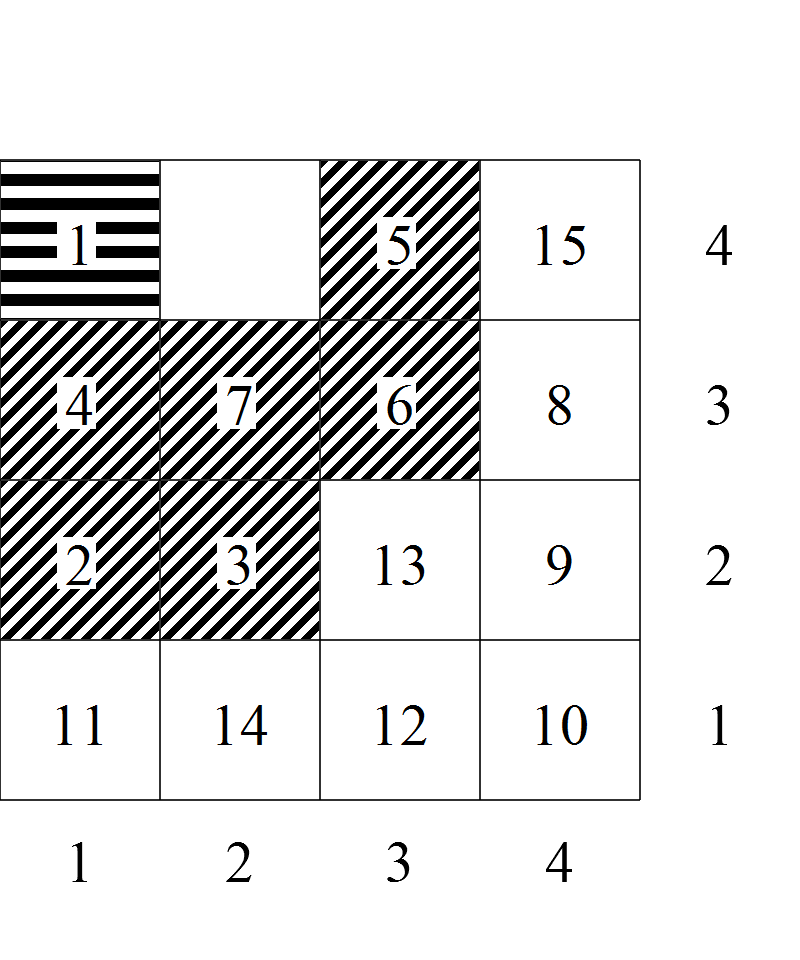
\includegraphics[width=\textwidth]{img/pre-solving-bsp-1.png}
    \caption{Das erste Bild}
    \label{fig:example:first:1st}
  \end{subfigure}
  \hfill
  \begin{subfigure}[t]{0.38\textwidth}
    \centering
    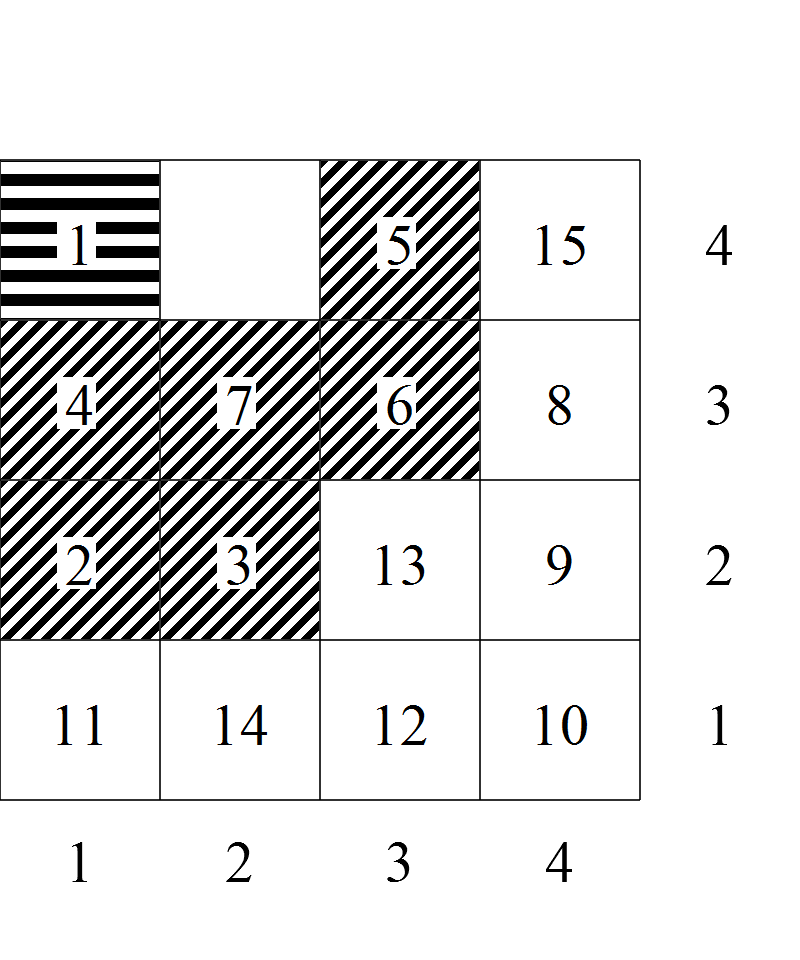
\includegraphics[width=\textwidth]{img/pre-solving-bsp-1.png}
    \caption{Das gleiche Bild, aber es könnte auch ein anderes sein!}
    \label{fig:example:first:2nd}
  \end{subfigure}

  \caption{Hier gibt es gleich zweimal was zu sehen.}
  \label{fig:example:first}
\end{figure}

Die ganze Abbilding hat das Label \texttt{fig:example:first} und kann dementsprechend mit
\texttt{\textbackslash{}ref\{fig:example:first\}} referenziert werden:
Abbildung~\ref{fig:example:first}.

Aber auch die enthaltenen \emph{Subfigures} haben ihre eigenen Label:
Abbildung~\ref{fig:example:first:1st} und Abbildung~\ref{fig:example:first:2nd}.
Diese Referenzen können auch in der Beschreibung der umgebenden Abbildung
benutzt werden um die Subabbildungen in Beziehung zueinander zu setzen.

\begin{figure}[htp]
  \centering
  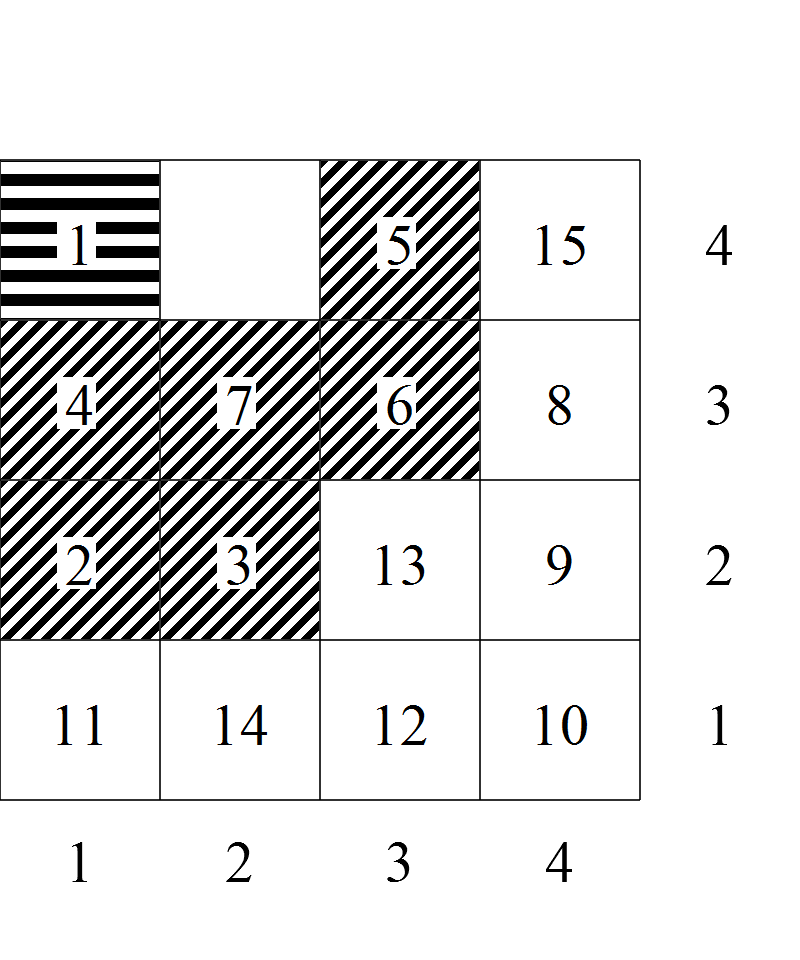
\includegraphics[width=0.3\textwidth]{img/pre-solving-bsp-1.png}
  \caption{Ein einzelnes Bild kann auch eingebunden werden...}
  \label{fig:einzeln}
\end{figure}


\paragraph{Bildformate}

Für Abbildungen~\ref{fig:example:first} wird eine PNG-Graphik
in das Dokument eingebunden.
Jedoch sollten Vektorgraphiken (PDF/SVG) gegenüber Rastergraphiken (PNG,GIF,JPG)
bevorzugt werden, da der Drucker und andere Ausgabegeräte selbstständig eine
angemessene Skalierung vornehmen können.




